% Options for packages loaded elsewhere
\PassOptionsToPackage{unicode}{hyperref}
\PassOptionsToPackage{hyphens}{url}
\PassOptionsToPackage{dvipsnames,svgnames,x11names}{xcolor}
\documentclass[
  10pt,
  fontset=fandol]{ctexart}
\usepackage{xcolor}
\usepackage[margin=16mm]{geometry}
\usepackage{amsmath,amssymb}
\setcounter{secnumdepth}{-\maxdimen} % remove section numbering
\usepackage{iftex}
\ifPDFTeX
  \usepackage[T1]{fontenc}
  \usepackage[utf8]{inputenc}
  \usepackage{textcomp} % provide euro and other symbols
\else % if luatex or xetex
  \usepackage{unicode-math} % this also loads fontspec
  \defaultfontfeatures{Scale=MatchLowercase}
  \defaultfontfeatures[\rmfamily]{Ligatures=TeX,Scale=1}
\fi
\usepackage{lmodern}
\ifPDFTeX\else
  % xetex/luatex font selection
\fi
% Use upquote if available, for straight quotes in verbatim environments
\IfFileExists{upquote.sty}{\usepackage{upquote}}{}
\IfFileExists{microtype.sty}{% use microtype if available
  \usepackage[]{microtype}
  \UseMicrotypeSet[protrusion]{basicmath} % disable protrusion for tt fonts
}{}
\makeatletter
\@ifundefined{KOMAClassName}{% if non-KOMA class
  \IfFileExists{parskip.sty}{%
    \usepackage{parskip}
  }{% else
    \setlength{\parindent}{0pt}
    \setlength{\parskip}{6pt plus 2pt minus 1pt}}
}{% if KOMA class
  \KOMAoptions{parskip=half}}
\makeatother
\usepackage{longtable,booktabs,array}
\newcounter{none} % for unnumbered tables
\usepackage{calc} % for calculating minipage widths
% Correct order of tables after \paragraph or \subparagraph
\usepackage{etoolbox}
\makeatletter
\patchcmd\longtable{\par}{\if@noskipsec\mbox{}\fi\par}{}{}
\makeatother
% Allow footnotes in longtable head/foot
\IfFileExists{footnotehyper.sty}{\usepackage{footnotehyper}}{\usepackage{footnote}}
\makesavenoteenv{longtable}
\usepackage{graphicx}
\makeatletter
\newsavebox\pandoc@box
\newcommand*\pandocbounded[1]{% scales image to fit in text height/width
  \sbox\pandoc@box{#1}%
  \Gscale@div\@tempa{\textheight}{\dimexpr\ht\pandoc@box+\dp\pandoc@box\relax}%
  \Gscale@div\@tempb{\linewidth}{\wd\pandoc@box}%
  \ifdim\@tempb\p@<\@tempa\p@\let\@tempa\@tempb\fi% select the smaller of both
  \ifdim\@tempa\p@<\p@\scalebox{\@tempa}{\usebox\pandoc@box}%
  \else\usebox{\pandoc@box}%
  \fi%
}
% Set default figure placement to htbp
\def\fps@figure{htbp}
\makeatother
\setlength{\emergencystretch}{3em} % prevent overfull lines
\providecommand{\tightlist}{%
  \setlength{\itemsep}{0pt}\setlength{\parskip}{0pt}}
\usepackage{amsmath,amssymb,mathtools,needspace}
\xeCJKDeclareCharClass{CJK}{"2032,"0400->"04FF,"2160->"216B,"2460->"2473,"25A0,"25C7,"25CB,"25CF}
\IfFontExistsTF{Arial Unicode MS}{\xeCJKsetup{AutoFallBack=true}\setCJKfallbackfamilyfont{\CJKrmdefault}{Arial Unicode MS}}{}
\setcounter{secnumdepth}{0}
\setlength{\emergencystretch}{2em}
\allowdisplaybreaks
\usepackage{bookmark}
\IfFileExists{xurl.sty}{\usepackage{xurl}}{} % add URL line breaks if available
\urlstyle{same}
\hypersetup{
  pdftitle={根的搜索},
  colorlinks=true,
  linkcolor={Maroon},
  filecolor={Maroon},
  citecolor={Blue},
  urlcolor={Blue},
  pdfcreator={LaTeX via pandoc}}

\title{根的搜索}
\author{}
\date{}

\begin{document}
\maketitle

\subsection{6.1 根的搜索}\label{ux6839ux7684ux641cux7d22}

数学、物理中的许多问题常常归结为求解函数方程 \(f(x)=0\)，这里，\(f(x)\) 可以是代数多项式，也可以是超越函数。方程 \(f(x)=0\) 的解 \(x^*\) 称为它的根，或称为 \(f(x)\) 的零点。

设函数 \(f(x)\) 在 \([a,b]\) 上连续，且 \(f(a)f(b)<0\)，根据连续函数的性质可知方程 \(f(x)=0\) 在区间 \((a,b)\) 内一定有实根，这时称 \([a,b]\) 为方程 \(f(x)=0\) 的有根区间。

\subsubsection{6.1.1 逐步搜索法}\label{ux9010ux6b65ux641cux7d22ux6cd5}

为明确起见，不妨假定 \(f(a)<0,f(b)>0\)。从有根区间 \([a,b]\) 的左端点 \(x_0=a\) 出发，按某个预定的步长 \(h\)（譬如取 \(h=\dfrac{b-a}{N}\)，\(N\) 为正整数）一步一步地向右跨，每跨一步进行一次根的``搜索''，即检查节点 \(x_k=a+kh\) 上的函数值 \(f(x_k)\) 的符号，一旦发现节点 \(x_k\) 与端点 \(a\) 的函数值异号，即 \(f(x_k)>0\)①，则可以确定一个缩小了的有根区间 \([x_{k-1},x_k]\)，其宽度等于预定的步长 \(h\)。

\textbf{例 6.1} 考察方程 \(f(x)=x^3-x-1=0\)。注意到 \(f(0)<0,f(2)>0\)，知 \(f(x)\) 在区间 \((0,2)\) 内至少有一个实根。

\textbf{解} 设从 \(x=0\) 出发，取 \(h=0.5\) 为步长向右进行根的搜索，列表记录各个节点上函数值的符号（见表 6.1），我们发现区间 \((1.0,1.5)\) 内必有一根。

表 6.1

{\def\LTcaptype{none} % do not increment counter
\begin{longtable}[]{@{}lllll@{}}
\toprule\noalign{}
\(x\) & \(0\) & \(0.5\) & \(1.0\) & \(1.5\) \\
\midrule\noalign{}
\endhead
\bottomrule\noalign{}
\endlastfoot
\(f(x)\) 的符号 & \(-\) & \(-\) & \(-\) & \(+\) \\
\end{longtable}
}

在具体运用上述方法时，步长 \(h\) 的选择是个关键。很明显，只要步长 \(h\) 取得足够小，利用这种方法可以得到具有任意精度的近似根。不过当 \(h\) 缩小时，所要搜索的步数相应增多，从而使计算量增大。因此，如果精度要求比较高，单用这种逐步搜索方法是不合算的。下述二分法可以看作逐步搜索方法的一种改进。

\subsubsection{6.1.2 二分法}\label{ux4e8cux5206ux6cd5}

再考察有根区间 \([a,b]\)，取中点 \(x_0=(a+b)/2\) 将它分为两半，然后进行根的搜

① 特别地，可能有 \(f(x_k)=0\)，这时 \(x_k\) 即为所求的根。

\href{../../source-images/pdf-156.jpeg}{原页}

索，即检查 \(f(x_0)\) 与 \(f(a)\) 是否同号，如果确系同号，说明所求的根 \(x^*\) 在 \(x_0\) 的右侧，这时令 \(a_1=x_0,b_1=b\)；否则 \(x^*\) 必在 \(x_0\) 的左侧，这时令 \(a_1=a,b_1=x_0\)（见图 6.1）。不管出现哪一种情况，新的有根区间 \([a_1,b_1]\) 的长度仅为 \([a,b]\) 的一半。

对压缩了的有根区间 \([a_1,b_1]\) 又可施行同样的手续，即用中点 \(x_1=(a_1+b_1)/2\) 将区间 \([a_1,b_1]\) 再分为两半，然后通过根的搜索判定所求的根在 \(x_1\) 的哪一侧，从而又确定一个新的有根区间 \([a_2,b_2]\)，其长度是 \([a_1,b_1]\) 的一半。

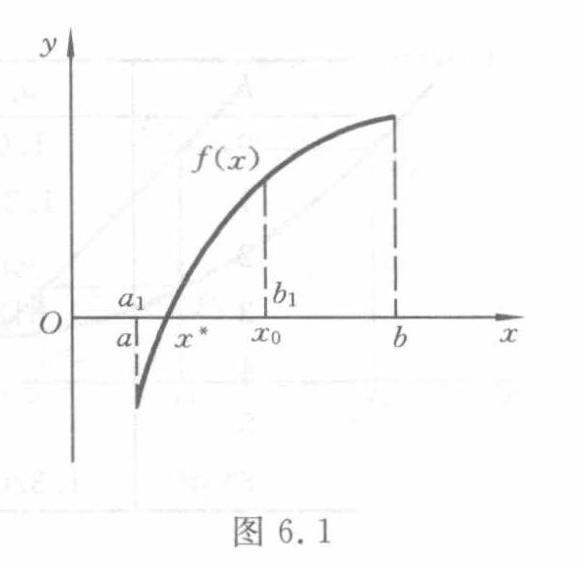
\includegraphics[width=0.85\linewidth,height=\textheight,keepaspectratio,alt={图 6.1 原扫描裁切}]{../assets/ch06/fig-6.1.png}

图 6.1

图意（agent 整理）：原图显示二分法的有根区间压缩。曲线标为 \(f(x)\)，坐标轴为 \(x,y\)，原点 \(O\)；横轴标有 \(a,x^*,x_0,b\)，新区间端点标有 \(a_1,b_1\)，其中 \(a_1=a,b_1=x_0\)。

如此反复二分下去，即可得出一系列有根区间

\[
[a,b]\supseteq[a_1,b_1]\supseteq[a_2,b_2]\supseteq\cdots\supseteq[a_k,b_k]\supseteq\cdots,
\]

其中每个区间都是前一个区间的一半，因此 \([a_k,b_k]\) 的长度 \(b_k-a_k=(b-a)/2^k\) 当 \(k\to\infty\) 时趋于零。就是说，如果二分过程无限地继续下去，这些区间最终必将收缩于一点 \(x^*\)，该点显然就是所求的根。

每次二分后，设取有根区间 \([a_k,b_k]\) 的中点 \(x_k=(a_k+b_k)/2\) 作为根的近似值，则在二分过程中可以获得一个近似根的序列 \(x_0,\allowbreak x_1,\allowbreak x_2,\allowbreak \cdots,\allowbreak x_k,\allowbreak \cdots\)，该序列必以根 \(x^*\) 为极限。

不过在实际计算时，不可能完成这个无限过程，其实也没有这种必要，因为数值分析的结果允许带有一定的误差。由于

\[
|x^*-x_k|\leqslant(b_k-a_k)/2=(b-a)/2^{k+1},
\]

只要二分足够多次（即 \(k\) 充分大），便有 \(|x^*-x_k|<\varepsilon\)，这里 \(\varepsilon\) 为预定的精度。

\textbf{例 6.2} 求方程 \(f(x)=x^3-x-1=0\) 在区间 \((1.0,1.5)\) 内的一个实根，要求准确到小数点后的第二位。

\textbf{解} 这里 \(a=1.0,b=1.5\)，而 \(f(a)<0,f(b)>0\)。取 \((a,b)\) 的中点 \(x_0=1.25\) 将区间二等分，由于 \(f(x_0)<0\)，即 \(f(x_0)\) 与 \(f(a)\) 同号，故所求的根 \(x^*\) 必在 \(x_0\) 右侧，这时应令 \(a_1=x_0=1.25,b_1=b=1.5\)，而得到新的有根区间 \([a_1,b_1]\)。

如此反复二分下去，二分过程无需赘述。现在预估所要二分的次数，按误差估计式（6.1.1），只要二分六次（\(k=6\)），便能达到预定的精度

\[
|x^*-x_6|\leqslant0.005.
\]

二分法的计算结果如表 6.2 所示。

二分法是电子计算机上一种常用算法，下面列出计算步骤：

\textbf{步 1} 准备。计算 \(f(x)\) 在有根区间 \([a,b]\) 端点处的值 \(f(a),f(b)\)。

\textbf{步 2} 二分。计算 \(f(x)\) 在区间中点 \(\dfrac{a+b}{2}\) 处的值 \(f\left(\dfrac{a+b}{2}\right)\)。

\begin{quote}
校注（agent 补充）：原页例 6.2 引用了``误差估计式（6.1.1）''，但本页对应的误差估计式旁未见印刷编号。此处保留原文引用及无编号公式，不补造公式标签；见 \href{../assets/ch06/detail-p156-audit.png}{误差估计式原图裁切}。
\end{quote}

\href{../../source-images/pdf-157.jpeg}{原页}

表 6.2

{\def\LTcaptype{none} % do not increment counter
\begin{longtable}[]{@{}lllll@{}}
\toprule\noalign{}
\(k\) & \(a_k\) & \(b_k\) & \(x_k\) & \(f(x_k)\) 符号 \\
\midrule\noalign{}
\endhead
\bottomrule\noalign{}
\endlastfoot
\(0\) & \(1.0\) & \(1.5\) & \(1.25\) & \(-\) \\
\(1\) & \(1.25\) & & \(1.375\) & \(+\) \\
\(2\) & & \(1.375\) & \(1.312\,5\) & \(-\) \\
\(3\) & \(1.312\,5\) & & \(1.343\,8\) & \(+\) \\
\(4\) & & \(1.343\,8\) & \(1.328\,1\) & \(+\) \\
\(5\) & & \(1.328\,1\) & \(1.320\,3\) & \(-\) \\
\(6\) & \(1.320\,3\) & & \(1.324\,2\) & \(-\) \\
\end{longtable}
}

\textbf{步 3} 判断。若 \(f\left(\dfrac{a+b}{2}\right)=0\) 则 \(\dfrac{a+b}{2}\) 即是根，计算过程结束。否则作如下检验：

若 \(f\left(\dfrac{a+b}{2}\right)\) 与 \(f(a)\) 异号，则根位于区间 \(\left(a,\dfrac{a+b}{2}\right)\) 内，这时以 \(\dfrac{a+b}{2}\) 代替 \(b\)；

若 \(f\left(\dfrac{a+b}{2}\right)\) 与 \(f(a)\) 同号，则根位于区间 \(\left(\dfrac{a+b}{2},b\right)\) 内，这时以 \(\dfrac{a+b}{2}\) 代替 \(a\)。

反复执行步 2 和步 3，直到区间 \([a,b]\) 长度缩小到允许误差范围之内，此时区间中点 \(\dfrac{a+b}{2}\) 即可作为所求的根。

二分法的优点是算法简单，而且收敛性总能得到保证。

\subsection{本节覆盖原页的校注记录}\label{ux672cux8282ux8986ux76d6ux539fux9875ux7684ux6821ux6ce8ux8bb0ux5f55}

下列记录按原页关联，含同页相邻小节的校注；计算时同时读取上文校注和完整原页。

\begin{itemize}
\tightlist
\item
  \texttt{ch06-E001}：原书 PDF 页 156
\end{itemize}

\end{document}
